\newpage
\section{Methods} \label{sec:methods}

As described above, to develop an algorithm to approximate the most likely spike train given fluorescence data, we first carefully analyze the statistics of typical data-sets.  We start by considering an in vitro experiment, for which the SNR is relatively high, and build an appropriate generative model (Section \ref{sec:model}).  Given this model, we can formally state our goal (Section \ref{sec:goal}).  And given this goal, we derive an approximately optimal inference algorithm (Section \ref{sec:inf}).  We then generalize our model in a number of ways, incorporating spatial filters (Section \ref{sec:spatial}), overlapping spatial filters (Section \ref{sec:overlap}), Poisson observations (Section \ref{sec:poisson}), fluorescence saturation (Section \ref{sec:satur}), and slow rise time for genetic sensors (Section \ref{sec:slow}).  Inferring the most likely spike train in all the above scenarios requires having an estimate of the parameters governing the relationship between the spikes and the movie.  Thus, we also develop an approach to efficiently approximate the maximum likelihood estimate (MLE) of the parameters (Section \ref{sec:learn}).  Finally, we describe several measures we use to assess and compare performance of our algorithm with others (Section \ref{sec:ass}).    

\subsection{Data driven generative model} \label{sec:model}

Figure \ref{fig:in_vitro_ex} shows a typical in vitro, epifluorescence data-set (see Section \ref{sec:exp} for data collection details).  The top panel shows a field-of-view, including 3 neurons, two of which are patched.  To build our model, we first define a region-of-interest (ROI),  which is this case is the circled neuron.  Given the ROI, we can average all the pixel intensities of each frame, to get a one-dimensional fluorescence time-series, shown in the bottom left panel (black line).  Because we are patched onto this neuron, we also know when this neuron is spiking (black bars). 
Previous work suggests that this fluorescence signal might be well characterized by convolving the spike train with an exponential, and adding noise \cite{ImagingManual}.  We confirmed that model for our data by convolving the true spike train with an exponential (gray line, bottom left panel), and then looking at the distribution of the residuals.  The bottom right panel shows (black line) a histogram of the residuals, and the best fit Gaussian distribution (gray line).


\begin{figure}[h!]
\centering 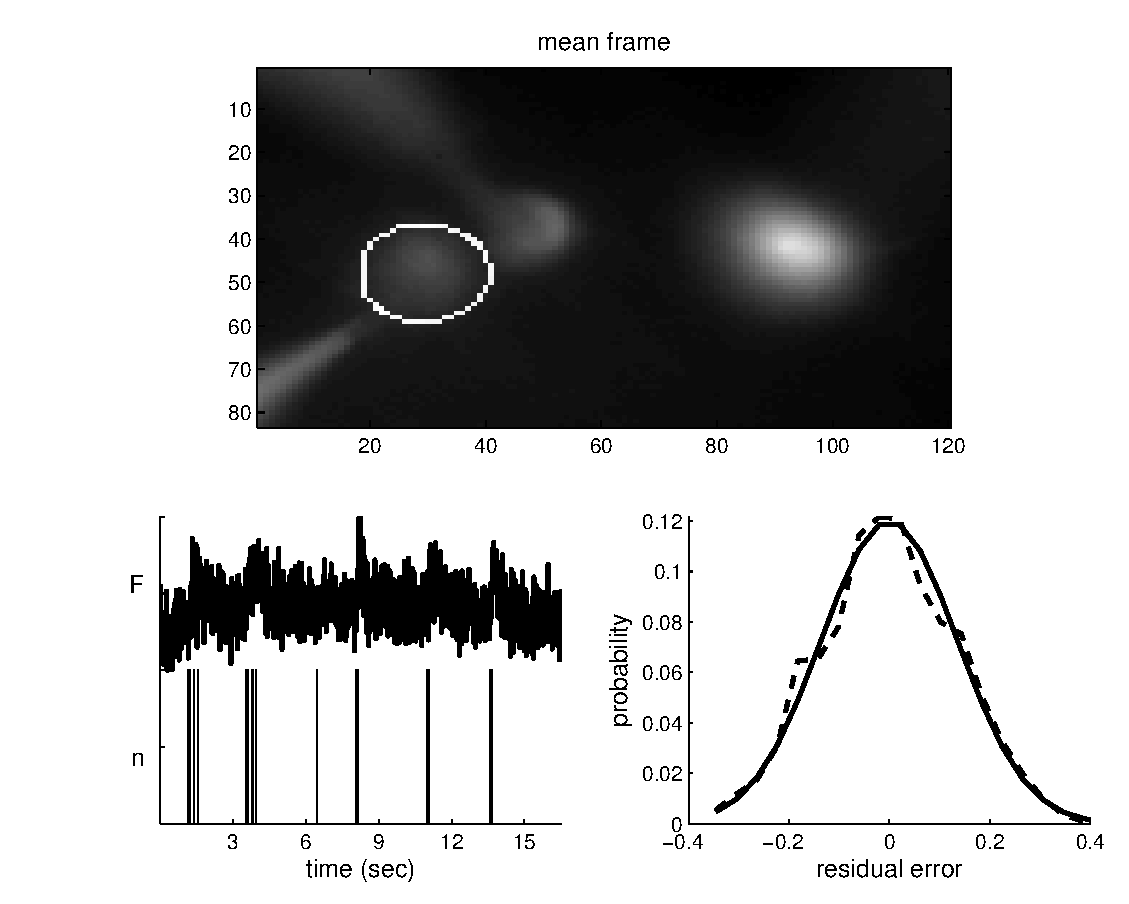
\includegraphics[width=.9\linewidth]{../figs/in_vitro_ex}
\caption{A typical in vitro data-set suggests that a reasonable first order model may be constructed by convolving the spike train with an exponential, and adding Gaussian noise. Top panel: the average (over frames) of a typical field-of-view.  Bottom left: spike train (black bars), convolved with an exponential (gray line), superimposed on the one-dimensional fluorescence time series (black line).  Bottom right: a histogram of the residual error between the gray and black lines from the bottom left panel (black line), and the best fit Gaussian (gray line).} \label{fig:in_vitro_ex}
\end{figure}

The above observations may be formalized as follows. Assume we have a 1-dimensional fluorescence trace, $\bF=(F_1, \ldots, F_T)$ from a neuron.  At time $t$, the fluorescence measurement, $F_t$ is a linear-Gaussian function of the intracellular calcium concentration at that time, $C_t$:

\begin{align} \label{eq:F}
F_t &= \alpha (C_t + \beta) + \sig \varepsilon_t, \qquad \varepsilon_t \overset{iid}{\sim} \mN(0,1)
\end{align}

\noindent The scale, $\alpha$, absorbs all experimental variables impacting the scale of the signal, including number of sensors within the cell, photons per change in intracellular calcium concentration per sensor, amplification of imaging system, etc.  Similarly, the offset, $\beta$, absorbs baseline calcium concentration of the cell, background fluorescence of the fluorophore, imaging system offset, etc.  The standard deviation, $\sig$, results from calcium fluctuations independent of spiking activity, fluorescence fluctuations independent of calcium, and imaging noise. The noise at each time, $\varepsilon_t$, is independently and identically distributed according to a standard normal distribution (i.e., Gaussian with zero mean and unit variance).  %These three parameters, and the Gaussianity of the noise,  correspond to a number of simplifying assumptions, that we will relax in Section \ref{sec:results}.  

We further assume that the intracellular calcium concentration, $C_t$, jumps after each spike, and subsequently decays back down to rest with time constant, $\tau$, yielding:

% $\tau (C_t-C_{t-1})/\Del = -C_{t-1} + n_t$.  Rearranging (and rescaling) a bit, we have:

\begin{align} \label{eq:C}
\tau \frac{C_t - C_{t-1}}{\Del} &= - C_{t-1} + n_t
\end{align}

\noindent where $\Del$ is the time step size --- which in our case, is the frame duration, or $1/$(frame rate) --- and $n_t$ indicates the number of times the neuron spiked at time $t$. %, and $\gam=1-\Del/\tau$. \footnote{This follows from writing \eqref{eq:C} as $\tau \frac{C_t - C_{t-1}}{\Del} = -C_{t-1} + n_t$.} 
Note that $C_t$ does not refer to absolute intracellular concentration of calcium but rather, a relative measure.  The assumed linearity of our model precludes the possibility of determining calcium in absolute terms (but see Section \ref{sec:nonlin} for a modified model).  The gray line in the bottom left panel of Figure \ref{fig:in_vitro_ex} corresponds to the putative $\bC$ of the observed neuron.  

To complete the ``generative model'' (i.e., a model from which we could generate simulations), we must also define the distribution from which spikes are sampled.  Perhaps the simplest first order description of spike trains is that at each time, spikes are sampled according to a Poisson distribution with some rate:

\begin{align} \label{eq:n}
	n_t \overset{iid}{\sim} \text{Poisson}(\lam \Del)
\end{align}

\noindent where $\lam \Del$ is the expected firing rate, and we have included $\Del$ to make $\lam$ be independent of the frame rate.  Thus, Eqs. \eqref{eq:F} -- \eqref{eq:n} complete our generative model.  






\subsection{Goal} \label{sec:goal}

Given the above model, our goal is to find the maximum \emph{a posteriori} (MAP) spike train, i.e., the most likely spike train, $\hbn$,  given the fluorescence measurements, $\bF$. Formally, we have:

\begin{align} \label{eq:nhat1} 
\hbn &=  \anx P[\bn | \bF], 
\end{align}

\noindent where $P[\bn | \bF]$ is the posterior probability of a spike train, $\bn$, given the fluorescent trace, $\bF$, and $n_t$ is constrained to be an integer ($\mathbb{N}_0=\{0,1,2,\ldots\}$).  From Bayes' Rule, we know that we can rewrite the posterior:

\begin{align} \label{eq:bayes}
P[\bn | \bF] = \frac{P[\bn, \bF]}{P[\bF]} = \frac{1}{P[\bF]} P[\bF | \bn] P[\bn],
\end{align}

\noindent where $P[\bF]$ is the evidence of the data; $P[\bF | \bn]$ is the likelihood of a observing a particular fluorescence trace $\bF$, given the spike train $\bn$, and $P[\bn]$ is the prior probability of a spike train.  Plugging Eq. \eqref{eq:bayes} into Eq. \eqref{eq:nhat1}, we have:

\begin{align} \label{eq:nhat2} 
\hbn &=  \anx \frac{1}{P[\bF]} P[\bF | \bn] P[\bn] =  \anx  P[\bF | \bn] P[\bn],
\end{align}

\noindent where the second equality follows because $P[\bF]$ merely scales the results, but does not change the relative quality of various spike trains.  Fortunately, both $P[\bF | \bn]$ and $P[\bn]$ are available from the above model:

\begin{subequations} \label{eq:post1}
\begin{align}
P[\bF | \bn]&= P[\bF | \bC] 	= \prod_t P[F_t | C_t], \label{eq:lik1} \\ 
P[\bn] 		&= \prod_t P[n_t], \label{eq:prior1}
\end{align}
\end{subequations}

\noindent where the first equality in Eq. \eqref{eq:lik1} follows because $\bC$ is deterministic given $\bn$, and the second equality follows from Eq. \eqref{eq:F}. Further, Eq. \eqref{eq:prior1} follows from the Poisson distribution assumption above, Eq. \eqref{eq:n}.  Fortunately, both $P[F_t | C_t]$ and $P[n_t]$ are given by the model:

\begin{subequations} \label{eq:post2}
\begin{align}
P[F_t | C_t] &= \mN(F_t; \alpha(C_t+\beta),\sig^2), \label{eq:lik2} \\
P[n_t] &= \text{Poisson}(n_t; \lam \Del). \label{eq:prior2} 
\end{align}
\end{subequations}

\noindent where $\mN(x;\mu,\sig^2)$ indicates $x$ has a Gaussian distribution with mean $\mu$ and variance $\sig^2$ and Poisson$(x;k)$ indicates that $x$ has a Poisson distribution with rate $k$, and both equations follow from the above model.  Now, plugging Eq. \eqref{eq:post2} back into \eqref{eq:post1}, and plugging that result into Eq. \eqref{eq:nhat2}, yields:

\begin{subequations}  \label{eq:obj}
\begin{align}
\hbn 	&= \anx \prod_t \frac{1}{\sqrt{2 \pi \sig^2}} \left(-\frac{1}{2}\frac{(F_t - \alpha (C_t + \beta))^2}{\sig^2}\right) \frac{\text{e}^{-\lam\Del} (\lam\Del)^{n_t}}{n_t!}
\label{eq:obj1}\\ &= \anx  \sum_t \bigg( -\frac{1}{2 \sig^2}(F_t - \alpha(C_t + \beta))^2  -  n_t \log \lam \Del + \log n_t! \bigg), \label{eq:logobj1}
\end{align} 
\end{subequations}

\noindent where the second equality follows from taking the logarithm of the right-hand-side.  Unfortunately, solving Eq. \eqref{eq:logobj1} exactly is computationally intractable, as it requires a nonlinear search over an infinite number of  possible spike trains.  We could restrict our search space by imposing an upper bound, $k$, on the number of spikes within a frame.  However, in that case, the computational complexity scales \emph{exponentially} with the number of image frames --- i.e., the number of computations required would scale with $k^T$ --- which for pragmatic reasons is intractable.  Thus, we approximate Eq. \eqref{eq:obj}, by modifying Eq. \eqref{eq:n}, replacing the Poisson distribution with an exponential distribution.  The advantage of this approximation is that the optimization problem becomes log-concave, meaning that we can use any gradient ascent method to guarantee that we achieve the global maximum (because there are no local maxima, other than the single global maximum).  The disadvantage, however, is that we lose the constraint of integer results, i.e., we allow for our answer to include ``partial'' spikes.  This ``disadvantage'' can be remedied by thresholding, or by considering the magnitude of a partial spike as the probability of a spike occurring in that time bin.  We discuss this in more detail in the Discussion section.





\subsection{Inference} \label{sec:inf}

Our goal here is to develop an algorithm to efficiently approximate $\hbn$, the most likely spike train, given the fluorescence trace. By letting Poisson$(n_t; \lam\Del) \approx$ Exponential$(n_t; \lam\Del)$, Eq. \eqref{eq:logobj1} becomes:

\begin{align} \label{eq:obj2}
\hbn &\approx \argmin_{n_t>0 \, \forall t}  \sum_{t=1}^T \bigg( \frac{1}{2 \sig^2}(F_t - \alpha(C_t + \beta))^2  + n_t \lam \Del \bigg) 
\end{align}

\noindent where the constraint on $n_t$ has been relaxed from  $n_t \in \mathbb{N}_0$ to $n_t \geq 0$ (since the exponential distribution can yield any non-negative number), and we replaced $\max$ with $\min$ and inverted the signs.  Note that this is a common approximation technique in the machine learning literature \cite{TBF01}, as the exponential distribution is the closest convex relaxation to its non-convex counterpart, the Poisson distribution. While this convex relaxation makes the problem tractable, the ``sharp'' threshold imposed by the non-negativity constraint prohibits the use of standard gradient ascent techniques \cite{CONV04}. We therefore take an ``interior-point'' (or ``barrier'') approach, in which we drop the sharp threshold, and add a barrier term, which must approach $-\infty$ as $n_t$ approaches zero (e.g., $-\log n_t$) \cite{CONV04}.  By iteratively reducing the weight of the barrier term, we are guaranteed to converge to the correct solution \cite{CONV04}.  Thus, our goal is to efficiently solve:
\begin{align} \label{eq:eta}
\hbn_{\zzz} &= \argmin_{n_t \forall t}  \sum_{t=1}^T \left( \frac{1}{2 \sig^2}(F_t - \alpha(C_t + \beta))^2  +  n_t  \lam \Del - \zzz \log(n_t) \right),
\end{align}
Since spikes and calcium are related to one another via a simple linear transformation, namely, $n_t= \del (C_t-\gam C_{t-1})$, where $\del=\tau/\Del$ and $\gam=1-\Del/\tau$.  Dropping $\del$ (because we have a free scale term) we may rewrite Eq. \eqref{eq:eta} in terms of $\bC$:

\begin{align} 
\hbC_{\zzz} &= \argmin_{C_t - \gamma C_{t-1} \geq 0 \forall t} \sum_{t=1}^{T} \left( \frac{1}{2 \sig^2} (F_t -\alpha (C_t + \beta))^2  + (C_t - \gamma C_{t-1}) \lam \Del - \zzz \log(C_t - \gamma C_{-1}) \right). \label{eq:eta2}
\end{align}

\noindent The concavity of Eq. \eqref{eq:eta2} facilitates utilizing any number of techniques guaranteed to find the global optimum.  The fact that the argument of Eq. \eqref{eq:eta2} is twice differentiable, allows for the use of the Newton-Raphson technique, which is typically more efficient than only incorporating the gradient \cite{CONV04}. First, we rewrite Eq. \eqref{eq:eta2} in matrix notation.  Note that we can write $\bM \bC = \bn$:

\begin{align} \label{eq:M}
\ve{M} \bC = %- \bb=
\begin{bmatrix}
1 & 0  & 0 & \cdots & \cdots \\
1 & -\gamma & 0 & \cdots & \cdots \\
0 & 1 & -\gamma & 0 & \cdots  \\
\vdots & \vdots & \vdots & \vdots & \vdots  \\
0 & 0 & 0 & 1 & -\gamma
\end{bmatrix}
\begin{bmatrix}
C_1 \\ C_2 \\ \vdots \\ \vdots \\ C_T  
\end{bmatrix}
= 
\begin{bmatrix}
n_1 \\ n_2 \\ \vdots \\ \vdots \\ n_T
\end{bmatrix}
= \bn
\end{align}

\noindent where $\ve{M} \in \mathbb{R}^{T \times T}$ is a bidiagonal matrix.  Then, leting $\ve{1}$ be a $T$ dimensional column vector and $\blam=\lam \Del \ve{1}\T$, we obtain: 

\begin{align} 
\hbC_{\zzz} 
&= \az  \frac{1}{2 \sig^2} \norm{\bF - \alpha (\bC +\beta)}^2 + (\bM \bC )\T \blam  - \zzz \log(\bM \bC)\T\ve{1},  \label{eq:eta3}
\end{align}

\noindent where $\bM \bC \geq \ve{0}$ indicates that every element of $\bM \bC$ is greater than or equal to zero, $\T$ indicates transpose, and $\log(\cdot)$ indicates an element-wise logarithm. Now, when using Newton-Raphson to ascend a gradient, we iteratively compute both the gradient, $\bg$ (first derivative), and Hessian, $\bH$ (second derivation), of the argument to be minimized, with respect to the variables of interest ($\bC_z$ here).  Then, we update our estimate, using $\bC_z \leftarrow \bC_z + s \bd$, where $s$ is the step size, and solving $\bH \bd = \bg$ provides $\bd$, the direction.  From Eq. \eqref{eq:eta3}, we therefore need:

\begin{subequations} \label{eq:NR}
\begin{align}
\ve{g} &= -\frac{\alpha}{\sig^2}(\bF -\alpha({\hbC\T}_{\zzz} + \beta)) + \ve{M}\T\blam - \zzz \ve{M}\T (\ve{M} \hbC_{\zzz})^{-1} \label{eq:g} \\
\ve{H} &= \frac{\alpha^2}{\sig^2} \ve{I} + \zzz \ve{M}\T (\ve{M} \hbC_{\zzz})^{-2} \ve{M} \label{eq:H}
\end{align}
\end{subequations}

\noindent where the exponents indicate element-wise operations. To compute $s$, we use ``backtracking linesearches'', meaning that we find the maximal $s$ that is (a) between $0$ and $1$ and (b) decreases the likelihood.

Typically, implementing Newton-Raphson requires inverting the Hessian, i.e., $\bd = \bH^{-1} \bg$, a computation that scales \emph{cubically} with $T$, i.e., requires approximately $T^3$ operations. Already, this would be a drastic improvement over the most efficient algorithm assuming Poisson spikes, which require $k^T$ operations (where $k$ is the maximum number of spikes per frame).  Here, because $\ve{M}$ is bidiagonal, the Hessian is tridiagonal, the solution may be found in approximately $T$ operations, via standard banded Gaussian elimination techniques (which can be implemented efficiently in Matlab using $\bH \backslash \bg$). In other words, the above approximation and inference algorithm reduces computations from exponential time to \emph{linear} time. We refer to this as the Fast Optimal OPtical Spike Inference (\foopsi) filter.





\subsection{Learning} \label{sec:learn}

In the above, we assumed that the parameters governing our model, $\vth=\{\alpha, \beta, \sig, \tau, \lam\}$, were known. In general, however, these parameters must be estimated from the data. Therefore, we take an approximate expectation-maximization approach for computing $\hbn$: (i) initialize some estimate of the parameters, $\hbth$, then recursively compute (ii) $\hbn$ using those parameters, (iii) update $\hbth$ given $\hbn$, and (iv) stop recursing when some convergence criteria is met.  The third step is described above; below, we provide details for each of the other steps.

\paragraph{Initializing the parameters}

Because the above model is linear, the scale of $\bF$ is arbitrary, so $\alpha$ can be fixed at $1$ without loss of generality.  The offset, however, is not arbitrary.  Because spiking is assumed to be sparse, $\bF$ tends to be around baseline, so we let $\beta$ be the mean of $\bF$.  $\sig$ is set to be the standard deviation of $\bF$.  Because previous work has shown that results are somewhat robust to minor variations in $\tau$ \cite{YaksiFriedrich06}, we initialize $\tau$ at 1 sec.  Finally, we let $\lam=10$ Hz, which is between typical baseline firing rates and evoked spike rate activity, for these data-sets.

\paragraph{Estimating the parameters given $\hbn$}

In the typical expectation-maximization setting, we find the parameters that maximize the expected value of the joint observed and hidden signals:

\begin{align} \label{eq:par1}
\hbth &= \argmax_{\bth} E_{P[\bF | \bC]} \log P[\bF, \bC | \bth].
\end{align}
In the above, however, we don't compute those expected values, rather, only the MAP estimate of the spike train and calcium trace.  Therefore, we approximate Eq. \eqref{eq:par1} by simply maximizing the parameters given the MAP estimate:

\begin{align} \label{eq:par2}
\hbth &\approx \argmax_{\bth} P[\bF| \hbC; \bth] P[\hbn | \bth]
\end{align}

\noindent where $\hbC$ is determined using the above described inference algorithm. The approximation in \eqref{eq:par1} is good whenever the likelihood is very peaky, meaning that most of the mass is around the MAP sequence.\footnote{The approximation in \eqref{eq:par1} may be considered a first-order Laplace approximation}   The argument from the right-hand-side of Eq \eqref{eq:par1} may be expanded: 

\begin{align} \label{eq:par2}
P[\bF| \hbC; \bth] P[\hbn | \bth] &= \prod_t P[F_t | \hC_t; \beta,\sig]  P[\hn_t | \lam].
\end{align}

\noindent where $\alpha$ is not present because of the arbitrary scale term, and $\tau$ is not present because it is not separable from $\hbn$. To estimate the remaining parameters, we have for $\beta$:

\begin{align}
	\hbeta &= \argmax_{\beta >0} \prod_t P[F_t | \hC_t; \beta,\sig] = \argmax_{\beta>0} \sum_t (F_t - (C_t + \beta))^2,
\end{align}

\noindent which is solved by letting $\hbeta=\langle \bF-\bC \rangle_t$, where $\langle \cdot \rangle_t$ indicates a mean over $t$.  $\sig$ is then the mean of the residuals, and $\hlam$ is the mean of $\hbn$. 

\paragraph{Convergence criteria}

We stop iterating the parameter update whenever (i) iteration number exceeds some upper bound, or (ii) relative change in likelihood does not exceed some lower bound.  In practice, we find that parameters tend to converge after several iterations, given our initialization. 


\subsection{Spatial filtering}

In the above, we implicitly assumed that the raw movie of fluorescence measurements collected by the experimenter had undergone two stages of preprocessing.  First, the movie was segmented, to determine regions-of-interest (ROIs).  This yields a vector, $\vF_t=(F_{1,t}, \ldots, F_{N_p,t})$, corresponding to the fluorescence intensity at time $t$ for each of the $N_p$ pixels in the ROI.  Second, at each time $t$, we projected that vector into a scalar, yielding $F_t$, the assumed input.  In this section, we determine the optimal projection.  Formally, we posit a more general model:

\begin{align} \label{eq:bF}
F_{x,t} &= \alpha_x (C_{x,t} + \beta) +  \sig \vec{\varepsilon}_{x,t}, \qquad &\varepsilon_{x,t} \sim \mathcal{N}(0,1)   
\end{align}

\noindent where $\alpha_x$ scales each pixel, from which some number of photons are contributed due to calcium fluctuations, $C_t$, and others due to baseline fluorescence, $\beta$.  Further, we have assumed that the noise is spatially and temporally white, with variance, $\sig^2$, in each pixel (an assumption that can be relaxed quite easily).  Performing inference in this more general model proceeds nearly identical as before. In vector notation, we have:

\begin{align} 
\hbC_{\zzz} 
&= \az  \frac{1}{2 \sig^2} \norm{\vec{\bF} - \valpha (\bC\T +\beta\ve{1}\T)}^2 + (\bM \bC )\T \blam  - \zzz \log(\bM \bC)\T\ve{1},  \label{eq:eta4}\\
\ve{g} &= -\frac{\valpha}{\sig^2}(\vbF -\valpha({\hbC\T}_{\zzz} + \beta)) + \ve{M}\T\blam - \zzz \ve{M}\T (\ve{M} \hbC_{\zzz})^{-1} \label{eq:g2} \\
\ve{H} &= \frac{\valpha\T \valpha}{\sig^2} \ve{I} + \zzz \ve{M}\T (\ve{M} \hbC_{\zzz})^{-2} \ve{M} \label{eq:H2}
\end{align}

\noindent where $\vbF$ is an $N_p$ by $T$ element matrix, $\valpha$ is column vectors of length $N_p$, and $\bI$ is an $N_p \times N_p$ identity matrix.  Typically, the spatial filter, $\valpha$ is unknown, and therefore must be estimated from the data.  In practice, we found that letting let $\valpha=\langle \vbF \rangle_t$ was both effective and extremely efficient.




\subsection{Overlapping spatial filters}

In the above, we assumed that the image was first segmented, such that only a single neuron was within each ROI.  However, segmentation is itself a difficult problem \cite{}.  Therefore, we would like to be able to use a crude segmentation technique, that might not actually produce ROIs with only a single cell, and then build spatial filters for each neuron in the ROI.  As before, this requires a minor modification to Eq.~\eqref{eq:bF}.  Specifically, letting the superscript $i$ index the $N_c$ neurons in this ROI, we obtain:  

\begin{align}
\vF_t &= \sum_{i=1}^{N_c}\valpha^i (C^i_t + \beta^i) +  \vec{\varepsilon}_t, \qquad &\vec{\varepsilon}_t \sim \mathcal{N}(\ve{0},\sig^2 \bI)   \\
C^i_t &= \gam^i C^i_{t-1} + n^i_t, & n^i_t \sim \text{Poisson}(n^i_t; \lam_i \Del)
\end{align}

\noindent where we have implicitly assumed that each neuron is independent, and that each pixel is independent and identically distributed with variance $\sig^2$.  To perform inference in this more general model, we define:

\begin{align} \label{eq:M2}
\bn &=  [n^1_1, n^2_1, \ldots, n^{N_c}_1, n^1_2, \ldots, n^{N_c}_T]\T \\
\bC &=  [C^1_1, C^2_1, \ldots, C^{N_c}_1, n^1_2, \ldots, C^{N_c}_T]\T \\
\ve{M} &= %- \bb=
\begin{bmatrix}
1 & 1 & 0 & 0 & \cdots & \cdots \\
1 & -\gam^1 & 1 & -\gam_2 & \ldots & 1 & -\gam_{N_c}  & 0 & \cdots \\
\vdots & \vdots & \vdots & \vdots & \vdots  \\
0 & 0 & 0 \ldots & 1 & -\gam^{N_c-1} & 1 & -\gam^{N_c}
\end{bmatrix}
\end{align} 

\noindent and proceed as above, making minor algorithmic adjustments to deal with dimensionality issues.  Since the parameters will be unknown, we must again estimate them. Letting $\balpha_x=[\alpha_x^1, \ldots, \alpha_x^{N_c}]\T$ and $\bbeta=[\beta^1, \ldots, \beta^{N_c}]\T$.  Assuming $\bbeta$ is known, we can estimate $\balpha_x$ using:

\begin{align}
\balpha_x = (\bC + \widetilde{\bbeta})\backslash \bF_x,
\end{align}

\noindent where $\widetilde{\bbeta}$ is $\bbeta$ reparameterized to be the same size as $\bC$.  Given this estimate of $\balpha_x$ for all $x$, we can then estimate $\beta^i=\norm{\vF - \valpha^i \bC^i}$.  In practice, iterating these two steps converged after several iterations, assuming enough spikes were present in the two neurons, and they were sufficiently uncorrelated.



















\subsection{Experimental Methods} \label{sec:exp}

\paragraph{Slice Preparation and Imaging}

All animal handling and experimentation was done according to the National Institutes of Health and local Institutional Animal Care and Use Committee guidelines. Somatosensory thalamocortical slices $400$ $\mu$m thick were prepared from C57BL/6 mice at age P14 as described \cite{MacLeanYuste05}. Neurons were filled with $50$ $\mu$M Fura $2$ pentapotassium salt (Invitrogen, Carlsbad, CA) through the recording pipette. Pipette solution contained $130$ K-methylsulfate, $2$ MgCl$_2$, $0.6$ EGTA, $10$ HEPES, $4$ ATP-Mg, and $0.3$ GTP-Tris, pH $7.2$ ($295$ mOsm).  After cells were fully loaded with dye, imaging was done by using a modified BX50-WI upright confocal microscope (Olympus, Melville, NY).  Image acquisition was performed with the C9100-12 CCD camera from Hamamatsu Photonics (Shizuoka, Japan) with arclamp illumination at $385$ nm and $510/60$ nm collection filters (Chroma, Rockingham, VT).  Images were saved and analyzed using custom software written in Matlab (Mathworks, Natick, MA).

\paragraph{Electrophysiology}

All recordings were made using the Multiclamp 700B amplifier (Molecular Devices, Sunnyvale, CA), digitized with National Instruments 6259 multichannel cards and recorded using custom software written using the LabView platform (National Instruments, Austin, TX) .  Waveforms were generated using Matlab and were given as current commands to the amplifier using the LabView and National Instruments system. The shape of the waveforms mimicked excitatory (inhibitory) synaptic inputs, with a maximal amplitude of $+70$ pA ($-70$ pA).